% !TEX root = ../../../main.tex
% 来源：中学数学实验教材·第二册（几何）
% 章节：集合与简易逻辑 / 简易逻辑
% 原始文件：2.tex，行 1776-1781
% 类型：tikz
% ---
    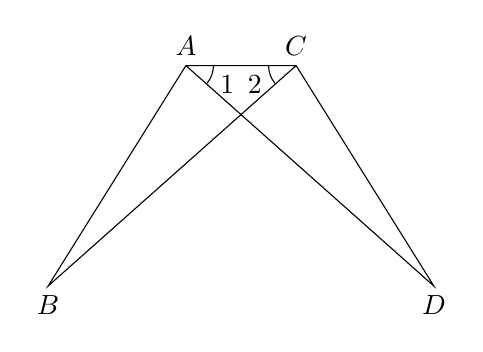
\begin{tikzpicture}[>=latex, scale=.7]
    \draw(1,0)--(-3.5,-4)node[below]{$B$}--(-1,0)node[above]{$A$}--(1,0)node[above]{$C$}--(3.5,-4)node[below]{$D$}--(-1,0);
	\draw (1-.5,0) arc (180:220:.5);
	\draw (-1+.5,0) arc (0:-40:.5);
	\draw(1-.75,0)node[below]{2};\draw(-1+.75,0)node[below]{1};
    \end{tikzpicture}
